\documentclass{minimal}
\usepackage{graphicx,color}
\usepackage[utf8]{inputenc}
\usepackage[papersize={418.00bp,314.00bp},text={418.00bp,314.00bp}]{geometry}
\begin{document}
\centering
% Title: Figure 2
% Creator: GL2PS 1.4.2, (C) 1999-2020 C. Geuzaine
% For: Octave
% CreationDate: Sun Aug 13 18:24:15 2023
\setlength{\unitlength}{1pt}
\begin{picture}(0,0)
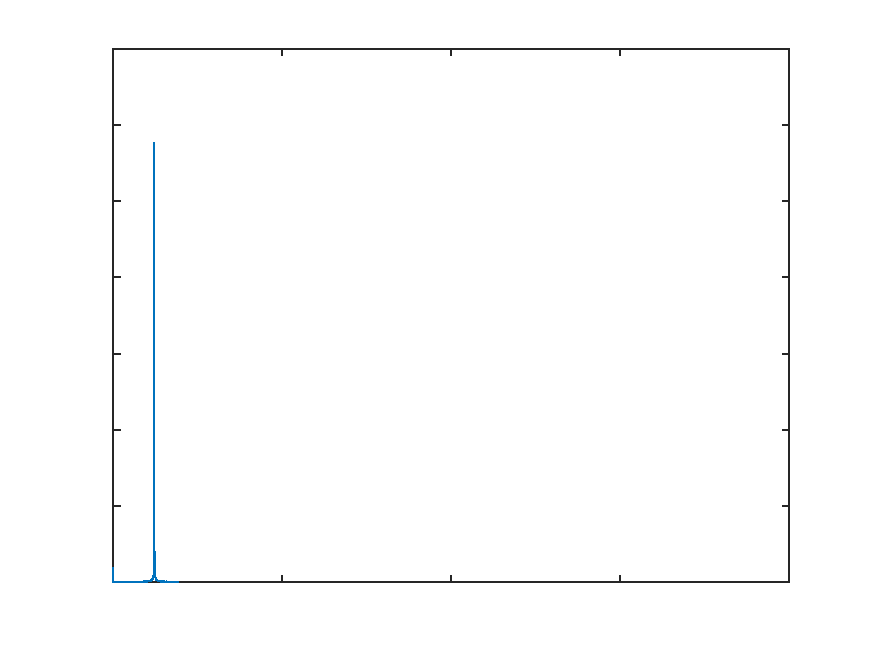
\includegraphics[scale=1]{plot15_7-inc}
\end{picture}%
\begin{picture}(418,314)(0,0)
\fontsize{10}{0}\selectfont\put(54.4343,27.0024){\makebox(0,0)[t]{\textcolor[rgb]{0.15,0.15,0.15}{{0}}}}
\fontsize{10}{0}\selectfont\put(135.562,27.0024){\makebox(0,0)[t]{\textcolor[rgb]{0.15,0.15,0.15}{{500000}}}}
\fontsize{10}{0}\selectfont\put(216.69,27.0024){\makebox(0,0)[t]{\textcolor[rgb]{0.15,0.15,0.15}{{1e+06}}}}
\fontsize{10}{0}\selectfont\put(297.818,27.0024){\makebox(0,0)[t]{\textcolor[rgb]{0.15,0.15,0.15}{{1.5e+06}}}}
\fontsize{10}{0}\selectfont\put(378.946,27.0024){\makebox(0,0)[t]{\textcolor[rgb]{0.15,0.15,0.15}{{2e+06}}}}
\fontsize{10}{0}\selectfont\put(49.4418,34.5008){\makebox(0,0)[r]{\textcolor[rgb]{0.15,0.15,0.15}{{0}}}}
\fontsize{10}{0}\selectfont\put(49.4418,71.0645){\makebox(0,0)[r]{\textcolor[rgb]{0.15,0.15,0.15}{{0.1}}}}
\fontsize{10}{0}\selectfont\put(49.4418,107.628){\makebox(0,0)[r]{\textcolor[rgb]{0.15,0.15,0.15}{{0.2}}}}
\fontsize{10}{0}\selectfont\put(49.4418,144.192){\makebox(0,0)[r]{\textcolor[rgb]{0.15,0.15,0.15}{{0.3}}}}
\fontsize{10}{0}\selectfont\put(49.4418,180.756){\makebox(0,0)[r]{\textcolor[rgb]{0.15,0.15,0.15}{{0.4}}}}
\fontsize{10}{0}\selectfont\put(49.4418,217.319){\makebox(0,0)[r]{\textcolor[rgb]{0.15,0.15,0.15}{{0.5}}}}
\fontsize{10}{0}\selectfont\put(49.4418,253.883){\makebox(0,0)[r]{\textcolor[rgb]{0.15,0.15,0.15}{{0.6}}}}
\fontsize{10}{0}\selectfont\put(49.4418,290.447){\makebox(0,0)[r]{\textcolor[rgb]{0.15,0.15,0.15}{{0.7}}}}
\fontsize{11}{0}\selectfont\put(216.69,14.0024){\makebox(0,0)[t]{\textcolor[rgb]{0.15,0.15,0.15}{{f (Hz)}}}}
\fontsize{11}{0}\selectfont\put(29.4418,162.474){\rotatebox{90}{\makebox(0,0)[b]{\textcolor[rgb]{0.15,0.15,0.15}{{|V(f)|}}}}}
\fontsize{11}{0}\selectfont\put(216.69,300.447){\makebox(0,0)[b]{\textcolor[rgb]{0,0,0}{{Single-sided amplitude spectrum}}}}
\end{picture}
\end{document}
